% Chapter Template

\chapter{Soluzione proposta} % Main chapter title

\label{Chapter6} % Change X to a consecutive number; for referencing this chapter elsewhere, use \ref{ChapterX}

\lhead{Capitolo 6. \emph{Soluzione proposta}} % Change X to a consecutive number; this is for the header on each page - perhaps a shortened title

%----------------------------------------------------------------------------------------
%	SECTION 1
%----------------------------------------------------------------------------------------

\section{Linguaggi}

Per l’implementazione del progetto sono stati utilizzati due linguaggi. Per tutta la parte con requisiti di mutua esclusione, accodamento e multithreading è stato utilizzato Ada, data la sua predisposizione di primitive a supporto della gestione dei thread e delle risorse protette, che hanno reso lo sviluppo più facile ed affidabile. Ad esempio l’implementazione delle risorse protette, la relativa mutua esclusione e l’accodamento sarebbero stati molto più complessi (e a rischio di errore) utilizzando un altro linguaggio.
Tutta la parte grafica (monitor e controller) non ha requisiti di concorrenza tra più thread, e per questo abbiamo deciso di utilizzare Java e le sue librerie grafiche (swing e awt). Questa scelta è stata dettata dalla facilità implementativa che Java offre nel reparto grafico, e anche dal desiderio di utilizzare l’occasione per imparare una delle librerie più utilizzate per la costruzione di GUI. Inoltre Java offre una portabilità maggiore, e associato a YAMI4 (anch’esso portabile) è sembrato un valore aggiunto dare la possibilità di portare il monitor ed il controller su altri PC senza la necessità di ricompilare, dato che sono le due entità che si prestano meglio ad essere usate in modalità “plug and play”.
\newpage
%----------------------------------------------------------------------------------------
%	SECTION 2
%----------------------------------------------------------------------------------------

\section{Componenti ad alto livello}

\begin{figure}[htbp]
	\centering
		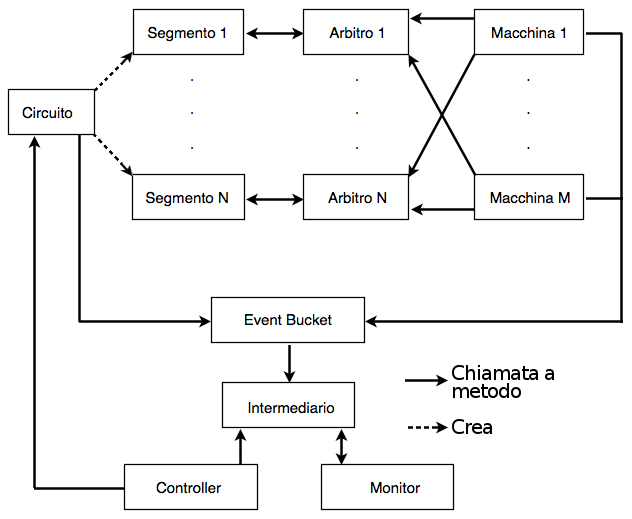
\includegraphics[keepaspectratio = true, width = 380px] {Pictures/schema}
		\rule{35em}{0.5pt}
	\caption[Componenti]{Componenti: visione ad alto livello delle componenti del sistema.}
	\label{fig:Componenti}
\end{figure}

\subsection{Circuito}

Come detto precedentemente il circuito viene rappresentato come una sequenza di segmenti. Ognuno di questi contiene le caratteristiche necessarie a descrivere il tratto associato: la lunghezza in metri, la molteplicità, ed un grado di difficoltà (da 1 a 10) che permette di discriminare le tipologie dei tratti (un rettilineo ha una difficoltà di 1, le curve variano da 2 a 10, a secondo dell’angolo descritto). Inoltre è stata aggiunta una variabile booleana per indicare se nel tratto è presente l’ingresso ai box.
All’interno del circuito è anche presente una entità attiva, che rappresenta il meteo. Questo task genera cambi casuali di tempo atmosferico, rendendo più realistica la gara, e generandone gli eventi relativi.
I dati relativi al tracciato vengono letti da un file “circuit.txt”, tramite un parser implementato ad hoc che processa le informazioni contenute nel file per costruire una struttura dati interna che si occupa di memorizzare tutte le informazioni necessarie.

\subsection{Arbitro}

L’arbitro è l’entità passiva che si interpone tra i veicoli ed un certo segmento. La sua utilità è molteplice, permette infatti di calcolare il tempo di attraversamento di un tratto dati i parametri della macchina, ed evita il formarsi di code di task in attesa per l’ingresso in un segmento fornendo subito una risposta. Possiamo dire che il vero lavoro di calcolo fisico della simulazione viene effettuato dall’arbitro, togliendo la possibilità alle macchine di autodeterminarsi.
I canali principali di questa entità sono due: la procedure “enterSegment” e “leaveSegment”, entrambe utilizzate dai task dei veicoli.
La prima viene chiamata quando una macchina richiede l’ingresso al segmento successivo a quello in cui si trova, e si affida all’arbitro per verificare la situazione ed agire di conseguenza.
Le possibilità sono due: se il numero di veicoli già presenti nel tratto è minore della molteplicità del medesimo (ad esempio se è vuoto), l’arbitro utilizzerà semplicemente i parametri del veicolo per calcolare la nuova velocità di uscita ed il tempo impiegato; in caso contrario, l’arbitro è obbligato a considerare il segmento saturo, e per questo dovrà sommare al tempo che la macchina avrebbe impiegato ad attraversare il tratto,  quello necessario a liberare il medesimo da un numero di veicoli sufficienti in modo che non possa più essere considerato saturo. Considerato che il tempo di uscita viene calcolato proprio dall’arbitro, è facile tenerne traccia per essere sempre a conoscenza di quando il tratto avrà posto disponibile. Anche nel secondo caso al termine del calcolo vengono restituiti alla macchina il tempo di attesa e la nuova velocità. Quest’ultima in questo caso sarà ridotta in modo da rispecchiare la decelerazione causata dalla presenza di una macchina che al momento non è superabile (data la saturazione della molteplicità).
In entrambi i casi la macchina è ignara dell’accaduto, nel senso che non sarà obbligata a restare in attesa su code o eseguire lavoro aggiuntivo.
Il secondo canale dell’entità arbitro, il “leaveSegment”, viene usato (come suggerito dal nome) per liberare il segmento da una macchina che ne è uscita. Dato che l’arbitro è a conoscenza dell’istante di uscita ogni veicolo, una scelta possibile sarebbe stata quella di non disporre questo secondo canale, e gestire tutto internamente all’arbitro. Il problema di questa scelta è dato dal fatto che quest’ultimo è un’entità passiva, ed è per questo impossibilitata ad effettuare controlli o ad intraprendere azioni attivamente. Inoltre dato che è la macchina l’entità attiva, ci è sembrato più sensato far compiere a lei le due azioni che implicano l’avanzamento della gara, cioè l’ingresso e l’uscita dal segmento. L’unico inconveniente che potrebbe sorgere è un possibile incremento ingiustificato del tempo di permanenza all'interno del segmento, causato dal fatto che “leaveSegment” è una procedure di una risorsa protetta, e quindi è in mutua esclusione con la procedure “enterSegment”; il problema è stato risolto imponendo by design che i veicoli non si risveglino contemporaneamente, ma sia sempre presente uno scarto temporale. L'algoritmo specifico verrà trattato successivamente.
Inoltre l’unica azione che viene compiuta dalla “leaveSegment” è quella di decrementare un contatore interno relativo al numero di macchine presenti nel segmento, che essendo una semplice operazione aritmetica viene eseguita senza sideeffects.


\subsection{Car}

Ogni vettura che partecipa alla gara è un’entità attiva separata. Ognuna è dotata di parametri propri, che cercano di rispecchiare le caratteristiche di un veicolo reale. Questi parametri vengono letti all’avvio del core, da un file “cars.txt” tramite parser. Dopo la lettura i task vengono creati utilizzando le informazioni lette dal file. Tra i parametri figurano velocità massima in $Km/h$, l’accelerazione in $m/s^2$, il comportamento del pilota (che implica la strategia), ed il suo identificativo. Inoltre sono presenti numerose altre informazioni che raffigurano lo stato in gara, come lo stato ed il tipo di gomme, i danni riportati in caso di incidente e la velocità istantanea.
Il ciclo di vita dei task macchina è relativamente semplice, infatti consiste nel richiedere l’ingresso in un segmento, attendere quanto specificato dall’arbitro, ed uscire dal segmento.
Questo ciclo viene ripetuto finchè i giri non terminano, o fino al ritiro del veicolo in caso di incidente.
L’attesa tra l’ingresso in un segmento e l’uscita dal medesimo viene fatta tramite il costrutto “delay until”, che ci assicura che in caso il risveglio del task ottenga qualche ritardo, quest’ultimo non venga accumulato al risveglio successivo.
Inoltre la macchina ha l’onere di generare gli eventi che la riguardano, come ad esempio l’uscita da un segmento o un incidente.

\subsection{Raccoglitore di eventi}

Data la grande mole di eventi generati durante la gara, sarebbe stato poco funzionale farli inviare all’intermediario direttamente dall’entità che li genera. Il rischio che si sarebbe corso è quello di rischiare di far perdere tempo ad un entità attiva, che è un comportamento poco desiderabile. Per questo abbiamo deciso di slegare completamente la creazione di un evento dalla sua distribuzione. Per farlo abbiamo creato un raccoglitore di eventi, o event bucket, che funziona con il classico paradigma produttore-consumatore; infatti ogni entità che produce eventi si occupa di inserirli in questo “secchio”, e sarà poi onere di qualcun altro consumarli adeguatamente.
Questa nuova figura è un’entità attiva che raccoglie gli eventi depositati e li invia all’intermediario tramite l’interfaccia di invio messaggi di yami4. Per evitare il busy-waiting è stato disposto un canale con guardia nel raccoglitore di eventi, in modo che il task di invio resti in attesa nell’entry finché la guardia non si apre (indicando la presenza di nuovi eventi da consumare) e li invia.
Scollegando la produzione dal consumo ci siamo assicurati che il funzionamento del sistema non sia dipendente da problemi esterni, come ad esempio malfunzionamenti della rete.

\subsection{Intermediario}

Il compito dell’intermediario è duplice, infatti oltre a dover comunicare con tutti gli altri nodi del sistema, ha anche il compito di elaborare gli eventi ricevuti dal core per renderli fruibili dall’utente attraverso il monitor.
In questo caso il problema da considerare non è banale, infatti ciò che viene ricevuto dal core è una sequenza di eventi, scanditi dal raggiungimento di alcuni obiettivi della gara (ovvero tempo in funzione dello spazio). Ciò che invece sarebbe auspicabile visualizzare per l’utente, è una sequenza continua che indica in ogni istante la situazione della gara, ovvero spazio in funzione del tempo. Quindi è necessario passare da informazioni basate sullo spazio (come una macchina che esce da un segmento) ad una rappresentazione temporale (uno snapshot di tutti i veicoli in un certo istante) come quello che si può vedere in TV durante le gare di F1.
L’intermediario ha quindi l’obbligo di interpolare i dati a disposizione per ricreare la situazione di gara, utilizzando i dati a disposizione (velocità, tempi di uscita, ecc…) per approssimare la posizione di ogni veicolo anche quando non ci sono informazioni disponibili (ad esempio quando la macchina è in attesa di uscire da un tratto).
Per questo vengono creati degli snapshot con una frequenza di mezzo secondo l’uno dall’altro, in cui sono contenute tutte le posizioni dei veicoli e la relativa situazione nella classifica; queste informazioni vengono inviate appena possibile ai monitor.
La creazione dello snapshot introduce anche un problema, infatti per rendere l’istantanea più corretta possibile, viene introdotta una breve latenza, in modo da permettere agli eventi attesi un piccolo margine di tempo per arrivare. Dato che gli eventi vengono salvati in alcune liste circolari, ed il tempo di esecuzione è relativo (ogni tempo si riferisce sempre all’istante zero) è stato introdotto un ritardo artificiale tra il tempo reale e quello dell’ultimo snapshot, creando un piccolo buffer logico che aumenta di molto la precisione delle previsioni effettuate. Tuttavia questo implica che il monitor visualizzerà la gara con ritardo di 1-2 secondi. Abbiamo comunque preferito procedere con questa soluzione perchè la latenza è costante, e può essere associata al problema reale del ritardo che intercorre tra l’invio delle immagini e la relativa ricezione e visualizzazione nella TV. Anche nel controller la cosa non ha un impatto problematico, infatti come detto precedentemente tutti i comandi che l’utente può comunicare non sono pensati per agire in tempo reale, ma essendo strategie posso soffrire di una breve latenza senza inficiarne le funzionalità.

\subsection{Monitor}

Il monitor ha la funzione di permettere all’utente di seguire graficamente lo svolgimento della gara. Come spiegato nel precedente paragrafo, tutte le informazioni vengono comunicate tramite snapshot al monitor, che le elabora costruendo una interfaccia di facile comprensione per l’utente.
La finestra che viene presentata è pensata per contenere i dati comuni a cui ogni utente è interessato, ed è quindi contenuta la rappresentazione grafica della gara e la classifica dinamica che riflette la situazione corrente dei partecipanti. In quest’ultimo elemento vengono anche incluse le informazioni più rilevanti relative ad ogni veicolo, come l’ingresso ai box o il verificarsi di incidenti.
Tutte le informazioni aggiuntive possono essere reperite dal controller.

\subsection{Controller}

Il controller permette di visualizzare informazioni aggiuntive su un certo veicolo, e dà la possibilità all’utente di modificare il comportamento del pilota (strategia) e di organizzare i rientri ai box. 
In linea teorica i dati ricavati dal controller non hanno bisogno di elaborazione, e quindi a differenza del monitor non soffrono della latenza necessaria alla creazione dello snapshot.
A questo punto è però sorto un problema, infatti il controller ed il monitor sono stati concepiti per essere utilizzati assieme, e non come elementi separati.  Senza pre-elaborazione dei dati aggiuntivi  nelle due finestre sarebbero stati presenti dati provenienti da due istanti leggermente diversi. Per rendere l’esperienza migliore, e considerato che la latenza è fissa e nota a priori, è stato deciso di aggiungere ai dati del controller lo stesso ritardo da cui sono affetti gli snapshot, in modo che le informazioni ottenute dalle due finestre siano perfettamente sincronizzate.

\section{Implementazione nel dettaglio}

Verrà ora descritta l’implementazione in modo dettagliato, per ogni package$/$classe più importante.
\begin{figure}[htbp]
	\centering
		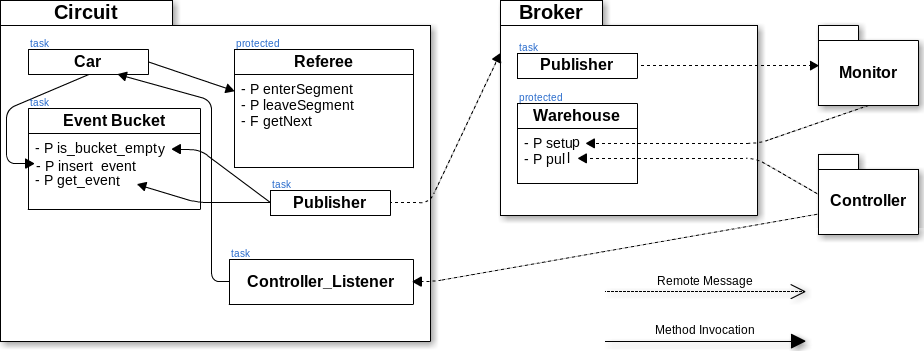
\includegraphics[keepaspectratio = true, width = 400px] {Pictures/SchemaOverview}
		\rule{35em}{0.5pt}
	\caption[Componenti]{Componenti: vista in dettaglio.}
	\label{fig:SchemaOverview}
\end{figure}

\subsection{Circuit}

Il package Circuit ha il compito di inizializzare tutte le componenti della simulazione. 
Il suo task bootstrap è responsabile di avviare la creazione della pista, attraverso un parser che legge le informazioni dei segmenti da un file di testo “circuit.txt”. Nel file di rappresentazione della pista sono presenti tante righe quanti sono i segmenti del tracciato, e ogni riga contiene cinque dati: l’identificatore del segmento, la lunghezza, la molteplicità, la difficoltà, e una variabile booleana che indica l’eventuale ingresso ai box.
Come spiegato precedentemente, le vere risorse protette sono rappresentate dall’arbitro, mentre i segmenti generati finora sono le descrizioni dei vari tratti. Sempre nell’inizializzazione, quindi, vengono creati gli arbitri, e ad ognuno viene assegnato il relativo tratto di competenza.
Un procedimento analogo viene fatto per le caratteristiche dei veicol, chei vengono anch’esse lette da un file di testo (cars.txt”, in cui ogni riga indica i parametri di una macchina; sono presenti quattro valori, l’id, il comportamento di default, la velocità massima, e l’accelerazione.
Per ogni riga viene creato un oggetto ``car\textunderscore status'' che verrà poi passato al task ``car\textunderscore p'' creato di conseguenza, che lo userà per leggere e salvare lo stato del veicolo rappresentato.
Le ultime cose che vengono effettuate nel bootstrap è l’inizializzazione e l’avvio del task “controller”, che predispone l’ascolto per l’override sul comportamento da parte dell’utente, ed il task publisher, che si occupa di inviare all’intermediario tutti i nuovi eventi.
Appena i task delle macchine vengono creati vengono messi in stato di sleep. Il tempo di risveglio è diverso fra le varie auto in modo da evitare l'accesso contemporaneo alla procedure del primo segmento . Senza di un controllo ogni macchina sarebbe partita appena creata, creando un vantaggio non controllabile dettato dallo scheduler per i primi veicoli inizializzati; in questo modo invece, le prime macchine create hanno un tempo di risveglio minore delle successive, creando una linea di partenza virtuale (basata sull’ordine dei veicoli indicati sul file di configurazione). Utilizzando questa soluzione il realismo della partenza viene rispettato, ed è implementato in modo che i task delle macchine non dovranno autonomamente controllare un flag ma saranno automaticamente svegliate dalla macchina astratta appena sarà il loro turno.
Dopo aver avviato la gara il task bootstrap si conclude.
Il Circuit contiene anche il task del meteo, che tramite la generazione di un numero casuale calcola un tempo di attesa prima del cambio di condizioni metereologiche. Per rendere più realistica questa componente, il tempo di attesa potrebbe essere anche più lungo del tempo totale di gara, implicando il mantenimento dello stesso stato per tutta la durata della competizione. Nell’attesa il thread è in stato di sleep, anche se viene risvegliato ogni 5 secondi per controllare se la gara è ancora in corso; questa condizione è stata resa necessaria per permettere la chiusura ordinata del programma, infatti è obbligatorio che il task controlli periodicamente se la competizione è terminata, chiudendosi assieme agli altri task in caso affermativo. Se non risvegliassimo il task del meteo ogni 5 secondi, ma ci limitassimo a svegliarlo solo quando deve cambiare stato, prima della chiusura del core dovremmo aspettare un tempo molto lungo e quindi proibitivo.

\subsection{Referee}

--TODO inserire flowchart entersegment in mezzo, SCIMMIA

Come ampiamente anticipato, il referee (o arbitro) è l’entità che incarna la vera risorsa protetta del segmento. 
Oltre al alcune funzioni e procedure necessarie per il setup, i canali principali che offre sono tre, “getNext”, “enterSegment”, “leaveSegment”.
La prima è una funzione rispecchia l’implementazione a linked list, in cui ogni elemento conosce solo i propri dati ed un puntatore all’elemento successivo.
La maggior parte del lavoro viene effettuata dalla procedure “enterSegment”, che ha l’onere di calcolare tramite vincoli fisici l’attraversamento del segmento da parte del veicolo o il suo ingresso ai box.
Per ricavare il tempo di attesa e la nuova velocità vengono utilizzate le leggi della cinematica modificate con coefficienti che alterano il risultato a seconda della strategia utilizzata dal pilota e dal tipo di tratto. Per quanto nella realtà l’accelerazione non sia costante, ci è sembrata una buona approssimazione, soprattutto considerando che il realismo fisico non è il fine ultimo del progetto.

\noindent%
\begin{minipage}{\linewidth}
\makebox[\linewidth]{%
  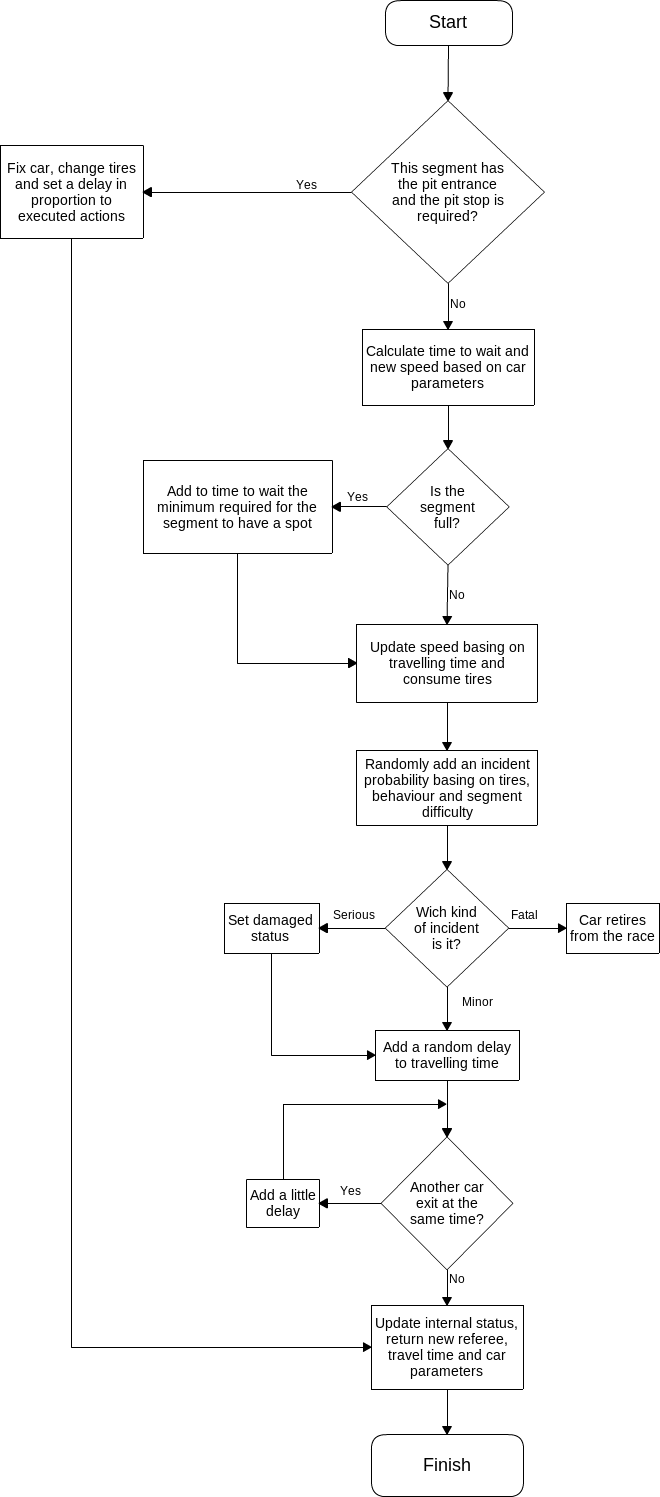
\includegraphics[keepaspectratio=true,scale=0.4]{Pictures/enterSegment}}
\captionof{figure}{Flowchart: procedure enterSegment.}% only if needed
\label{enterSegment}
\end{minipage}

Dopo aver calcolato il tempo di attesa e la nuova velocità del veicolo, viene effettuato un controllo sulla molteplicità del tratto, verificando il numero di veicoli al momento presenti all’interno. In caso ci sia spazio per un’altra macchina, il tempo e la velocità restano invariate, dato che rappresentano il massimo che la vettura può ottenere; in caso contrario la vettura deve accodarsi alla più vicina che la precede, e viene quindi sommato al tempo di uscita del veicolo il minor tempo per permettere l’uscita di una delle macchine già presenti.
Essendo in possesso del nuovo tempo di uscita viene ricalcolata la velocità, simulando la frenata necessaria ad adeguarsi al veicolo che la precede.
L’arbitro provvede anche ad aggiornare lo stato delle gomme dei veicoli, calcolandone il consumo basato sul tratto percorso, sul comportamento del pilota, ed in piccola parte dalla casualità (che aggiunge una piccola parte di non determinismo). La variabile che rappresenta lo stato attuale delle gomme viene utilizzata per eseguire il rientro ai box per il cambio gomme quando quest’ultime sono troppo usurate.
Successivamente viene calcolata la probabilità di incidente, che si basa su un calcolo che utilizza sia elementi casuali che coefficienti riguardanti lo stato della pista, il comportamento del pilota, il meteo, e l’adeguatezza delle gomme alla situazione atmosferica. La probabilità di incidente in uscita dal segmento varia dallo 0.1\% in condizioni favorevoli, allo 0.4\% in condizioni difficili.
In caso di uscita è presente un 10\% di probabilità di danneggiamento del veicolo, e un 5\% di probabilità di rottura irrimediabile che causi il ritiro.
Il referee ha inoltre il dovere di gestire l’ingresso ai box nel caso sia proprietario di un tratto con ingresso al pit stop. I box non sono rappresentati da un vero segmento, ma sono invece espressi da uno stato logico; quando l’arbitro deve far entrare un veicolo ai box agisce diversamente, calcolando un tempo di uscita basato sulla necessità di riparazioni o il semplice cambio gomme. E’ stato scelto di non creare una tipologia diversa di segmento per la gestione del box perché dato che l’output resta sempre il tempo di attesa e la velocità di uscita, avremmo creato qualcosa di nuovo per gestire una azione che viene già supportata dal referee. La soluzione che abbiamo adottato è quindi di far calcolare il tempo di uscita in base alle azioni intraprese nei box (cambio gomme/riparazioni) e restituire alla macchina il segmento di uscita dai box invece che quello successivo. Quando alla macchina sarà comunicato il nuovo stato genererà un evento relativo ai box invece che quello relativo ad un semplice segmento.

\subsection{Car}

--TODO flowchar ciclo di vita car, SCIMMIA

Il task Car, contenuto nel package car\textunderscore p, è ciò che rappresenta il funzionamento di una macchina che partecipa alla competizione.
Il suo ciclo di vita consiste in due azioni principali, la richiesta di ingresso in un segmento, e l’applicazione delle istruzioni restituite dal referee.
Per la prima, viene utilizzata l’entry “enterSegment” del referee, a cui vengono passati i parametri attuali, e si aspetta in uscita i dati neccessari a proseguire, cioè il tempo di attesa, un puntatore al prossimo arbitro da contattare, ed il nuovo stato del veicolo.
A questo punto il task deve controllare i dati restituiti, ed agire di conseguenza. I casi possono essere molteplici, e per questo deve generare gli eventi necessari per spiegare l’andamento di una gara, comunicando un eventuale incidente (con possibili danni o ritiro), il rientro ai box, o la semplice uscita del segmento (associata alla nuova velocità, strategia e gli altri dati necessari all’intermediario).
Il tempo di attesa è stato implementato con un “delay until”, che a differenza del semplice “delay” permette di ottenere una precisione migliore e non causa latenza incrementale. Per questo è stato necessario avere un riferimento assoluto di tempo. La scelta è stata quella di leggere il clock del PC solo una volta, all’avvio del task, e sommare di volta in volta il tempo di attesa derivante dall’attraversamento del segmento.
In questo modo anche se la macchina dovesse impegare del tempo per inviare gli eventi al raccoglitore, o se venisse svegliata più tardi di quanto richiesto, non accumulerebbe alcuna latenza, dato che il momento del risveglio è già stato fissato, ed il tempo di elaborazione è molto più piccolo di quello di attesa.

--TODO dimostrazione, SCIMMIA
Questo lo si può dimostrare nel seguente modo:

Un’altra scelta possibile sarebbe stata quella di far inviare gli eventi direttamente dall’arbitro, ma aggiungere del lavoro all’interno di una risorsa protetta ci è sembrata una cattiva idea in quanto poteva tranquillamente occuparsene un task durante le attese.
Al risveglio la macchina provvede ad avvisare l’arbitro della sua uscita dal segmento, e continua il ciclo finchè non terminano i giri, o un incidente la costringe al ritiro. In entrambi i casi, prima di concludere il task, la vettura comunica all’entità che mantiene lo stato della gara la sua uscita dalla competizione, in modo che quando non ci sarà più nessun veicolo in corsa potrà comunicare la fine della simulazione e chiudere in modo ordinato.
Oltre alla comunicazione degli eventi la macchina si occupa anche di compiere alcune operazioni di default, come programmare il rientro ai box per il cambio gomme in caso di pioggia o di usura, o in caso di danneggiamento di conseguenza ad un incidente. La sosta ai box può anche essere programmata dall’utente, facendo override sul comportamento di default della macchina.

\subsection{Event Bucket}

L’event bucket è una risorsa protetta presente all’interno del package event\textunderscore bkt. Il suo scopo è quello di raccogliere gli eventi provenienti dalle varie entità del core, e renderle disponibili ad un task che le invii all’intermediario.
Come già anticipato, la sua funzione è quella di “magazzino”, in cui i produttori mettono gli eventi in attesa che il consumatore li raccolga, ed è stato implementato per permettere la separazione logica tra chi produce e chi consuma, non obbligando il contatto diretto (che comporta possibili perdite di tempo).
All’inizializzazione viene definita la sua capacità, che deve essere abbastanza ampia per gestire la raccolta di eventi in rapida successione.
Le funzioni principali si raggiungono con tre canali, “insert\textunderscore event”, “get\textunderscore event” e “is\textunderscore bucket\textunderscore empty”.
La procedura “insert\textunderscore event” viene chiamata da tutti i produttori, e serve ad inserire l’evento all’interno del bucket. Ogni evento è rappresentato da un array di stringhe, contenente i vari dati relativi. Il bucket invece, è stato implementato come un vector, data la sua predisposizione ad essere gestito come una coda FIFO. All’inserimento di ogni evento un contatore aumenta, tenendo sempre conto del numero di elementi non ancora consumati.
L’entry “get\textunderscore event” restituisce il primo elemento della coda, e diminuisce il contatore degli eventi. All’ingresso di questa entry è stata posta una guardia, che si apre solo quando è presente almeno un elemento.
La procedura “is\textunderscore bucket\textunderscore empty” restituisce un valore booleano che indica se il bucket è vuoto; la sua necessità risulta evidente nel momento di chiusura dei task a termine della gara, infatti se il task di invio terminasse solo perché ogni veicolo ha raggiunto il termine, potrebbe non inviare gli ultimi eventi in coda, e per questo la terminazione è basata anche sulla quantità di eventi rimanenti.

\subsection{Publisher}

Il publisher si occupa di “impacchettare” i messaggi ed inviarli al broker. Come detto precedentemente, i messaggi vengono salvati nel broker come array di stringhe, mentre il messaggio che verrà inviato è implementato come una lista di coppie chiave/valore.
Ogni evento è identificato dall’attributo type, che può essere di otto tipi:

\begin{itemize}
 \item Eventi generati dai veicoli
 \begin{itemize}
  \item ES indica l’uscita da un segmento
  \item EB indica l’ingresso ai box
  \item LB indica l’uscita dai box
  \item EL indica la fine di un giro
  \item CE indica la fine della gara
  \item CA indica un incidente
 \end{itemize}
 \item ER indica la fine della gara
 \item SE indica il setup
\end{itemize}

Il primo compito è quello di recuperare gli eventi dal bucket, e convertirli da array di stringhe a liste di coppie. Ogni tipo di evento ha un numero fissato di parametri da contenere, quindi durante la conversione deve esclusivamente controllare la tipologia di evento per sapere come procedere.
Una volta creato l’evento viene inviato immediatamente al broker.

\subsection{Broker}
TOODO inserisci flowchart brokersnapshot, SCIMMIA

Il broker, o intermediario, si occupa di mediare la comunicazione fra il core principale che esegue la simulazione, e gli eventuali monitor o controller che vogliono visualizzarne lo stato in un dato istante. Ottiene il duplice scopo di bilanciare il traffico di rete e di processare i dati forniti dal simulatore in modo che siano più facilmente fruibili per la visualizzazione. Infatti, ponendosi a metà tra monitor e core, permette di alleggerire il carico di lavoro del simulatore poichè la comunicazione di quest’ultimo sarà sempre solo con un entità singola (il broker), indipendentemente dal numero di monitor che stanno visualizzando la gara in un dato istante.
Come prima cosa apre un canale di comunicazione che il core utilizzerà per inviare gli eventi man mano che vengono prodotti, tramite un architettura push. Gli eventi vengono smistati in base al loro tipo, e memorizzati nello stato interno del broker utilizzando una lista circolare. In questo modo riusciamo a mantenerne uno storico. L’utilizzo di una lista circolare è stato dettato dal fatto che per ragioni di memoria limitata non possiamo memorizzarli tutti. In questo modo quando lo spazio è esaurito gli eventi più recenti vengono sempre memorizzati, ricavando spazio dalla rimozione di quelli più obsoleti.
Gli eventi così memorizzati vengono poi elaborati in modo da ricavare uno snapshot, ovvero una “fotografia” della gara in un dato istante, fruibile dal monitor per la visualizzazione. Questo è necessario perchè gli eventi generati dal core si riferiscono al dominio dello spazio, ma per poter essere fruibili da un utente umano è necessario che essi siano nel dominio del tempo.
La costruzione dello snapshot viene effettuata ripetutamente a intervalli discreti e regolari.
Gli eventi ricevuti dal monitor contengono tutti un timestamp, ovvero il tempo in millisecondi relativo dall’inizio della simulazione in cui sono stati generati. La maggior parte di essi contiene anche il numero identificativo della macchina che li ha prodotti. Grazie a questi due campi è possibile raggruppare eventi che si riferiscono alla stessa macchina, e ordinarli in base al timestamp in modo crescente.
Quanto generiamo uno snapshot, fissiamo un tempo t e cerchiamo nella lista di eventi di ogni macchina gli eventi che corrispondono al timestamp precedente e immediatamente successivo.
Analizzando questi due eventi riusciamo a determinare dove si troverà (o meglio, dove si trovava) la macchina al tempo t fissato. Utilizzando i dati forniti degli eventi trovati, calcoliamo la posizione della macchina e la memorizziamo nello stato interno sovrascrivendo lo stato precedente. Una volta effettuata questa operazione per tutte le macchine appartenenti al sistema, siamo in grado di determinare la posizione in classifica di ogni macchina per quel dato istante. Aggiungiamo questa informazione allo stato interno e copiamo il tutto all’interno di una risorsa protetta che verrà usata per passare queste informazioni ai monitor/controller. L’utilizzo di una risorsa protetta è stato reso necessario dal fatto che le informazioni vengono prelevate in modo concorrente, e vogliamo quindi assicurarci che lo snapshot fornito sia completo e coerente.
Gli snapshot vengono suddivisi in due categorie: lo snapshot dettagliato e quello generalista. Lo snapshot dettagliato contiene informazioni aggiuntive per ogni macchina, come ad esempio la velocità corrente o lo stato attuale delle gomme. Queste informazioni non sono necessarie per la rappresentazione del monitor, e vengono quindi salvate in una risorsa protetta separata da quella che contiene lo snapshot generalista.
Lo snapshot che contiene i dati necessari per visualizzare lo stato della gara in un dato istante viene inviato tramite Publish a tutti  i monitor che sono interessati. Lo snapshot dettagliato viene invece richiesto tramite Pull dal controller.
Anche in questo caso l’insieme degli snapshot generati viene raccolto in un bucket, in modo da disaccoppiare il produttore dai consumatori. 
Il consumatore, ovvero l’entità che prende gli snapshot dal bucket e li invia ai monitor, è un task chiamato “updater”. Questo task viene creato durante il bootstrap del broker, e viene assegnato ad una porta secondo l’argomento passato come parametro, sulla quale farà il publish dello snapshot ogni volta che ne viene creato uno nuovo.
Per l’invio degli snapshot dettagliati viene invece creata un entità attiva chiamata “broker\textunderscore warehouse” che agisce da pull server: si mette in ascolto su una porta (anch’essa decisa come parametro) e invia i dati ogni volta che vengono richiesti.

\subsection{Monitor}

\begin{figure}[htbp]
	\centering
		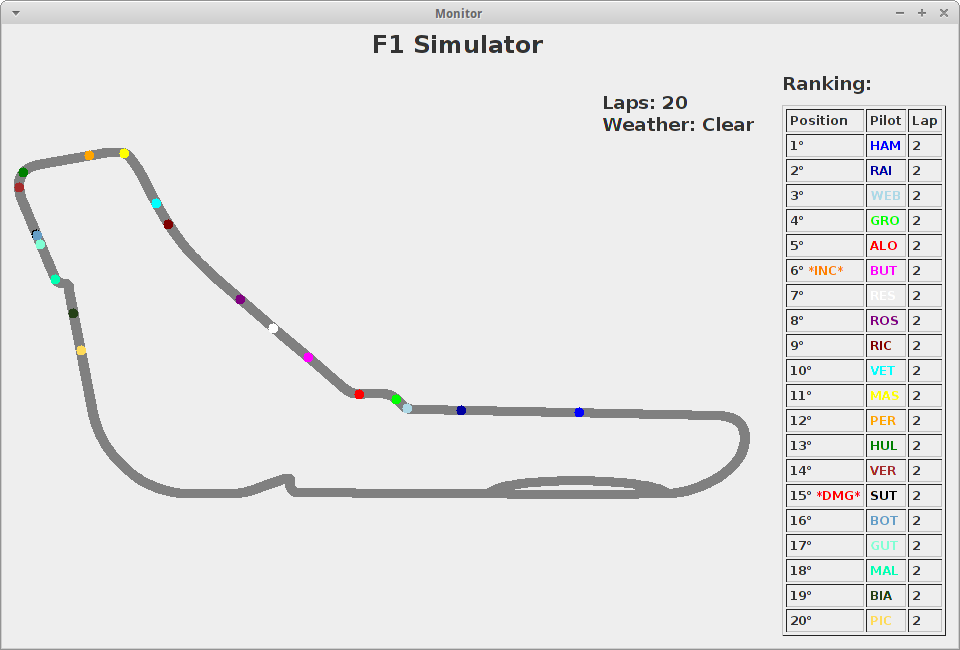
\includegraphics[keepaspectratio = true, width = 380px] {Pictures/monitor}
		\rule{35em}{0.5pt}
	\caption[Monitor]{Monitor: Rappresentazione della pista con classifica.}
	\label{fig:Monitor}
\end{figure}

Come anticipato, il monitor è l’elemento che permette all’utente di vedere in modo chiaro ed immediato l’andamento della gara.
Il monitor contiene due elementi fondamentali, la classifica (con gli stati attuali delle vetture) e la rappresentazione grafica dello stato della pista. Quest’ultima si basa sui dati ottenuti dal broker, ma non si limita a visualizzarli semplicemente a schermo, ma viene prima effettuata una seconda interpolazione per permettere di rendere fluida l’animazione del movimento dei veicoli.
Il setup del monitor reperisce informazioni da più fonti, infatti viene effettuato un pull di dati dal broker per il numero dei giri e di veicoli, mentre tutto quello che riguarda specifiche ulteriori (di visualizzazione) è contenuto nei file di configurazione. L’oggetto Drivers (Drivers.java) si occupa di leggere i dati contenuti nel file “carsProp.txt”, in cui sono contenute le informazioni riguardanti i nomi dei piloti ed il colore del loro veicolo. Abbiamo scelto di mantenere queste informazioni separate dal core perché non sono necessarie al funzionamento del simulatore, e avrebbero implicato un numero maggiore di informazioni da inviare tra i vari nodi del sistema distribuito. Inoltre in questo modo l’utente può personalizzare i colori ed i nomi dei piloti che vengono visualizzate sul monitor di cui dispone.
Successivamente deve essere letta e creata la pista; il file che viene utilizzato dal core per la creazione dei segmenti non è sufficiente, dato che include solo i dati necessari alla simulazione fisica, ma non spiega la forma del tracciato. Per questo motivo il file contenente la mappa del circuito è separato. Ogni segmento del circuito viene rappresentato come un oggetto con interfaccia Segment (Segment.java), che è stato implementato da due classi, StraightSegment e TurnSegment. Come intuibile dal nome il primo rappresenta un segmento rettilineo, mentre il secondo una curva. Ogni Segment offre la funzione getPosition, che data la percentuale di avanzamento del segmento restituisce la posizione in pixel in cui è presente il veicolo. Per quanto la funzione sia la stessa per i due tipi di segmento, la loro implementazione è profondamente diversa.
I segmenti rettilinei vengono inizializzati tramite quattro variabili intere, che rappresentano relativamente il punto di inizio del segmento ed il punto di fine. Data la percentuale di percorrenza, è facile utilizzare una proporzione in centesimi per ricavare la posizione corrente all’interno del tratto.
La situazione è differente per le curve, infatti abbiamo dovuto cercare un metodo per rappresentarle che fosse preciso, flessibile, ed impostabile manualmente (per permettere ad un utente di creare il proprio circuito). La prima idea è stata quella di definire solo alcuni tipi di curve possibili, e collegarle con i segmenti, in modo da assemblare la pista con una serie di “pezzi” possibili. Il problema di questa soluzione è che inevitabilmente avrebbe tolto la possibilità di riprodurre un tracciato reale esistente, caratteristica piuttosto importante per ogni appassionato di F1.
Quindi abbiamo cercato un modo per rendere la rappresentazione più fedele alla realtà, e di conseguenza abbiamo cercato di affidarci a formule matematiche ad hoc per ogni curva, ma come è facilmente intuibile questa soluzione è tutt’altro che pratica per la costruzione manuale di un tracciato.
La soluzione che abbiamo adottato, è quella che viene spesso utilizzata nei software di computer grafica, cioè l’utilizzo delle curve di Bézier; queste curve parametriche vengono definite da un numero variabile di punti intermedi, che ne specificano la concavità. Nel nostro caso abbiamo utilizzato delle curve cubiche, cioè caratterizzate da quattro punti (gli estremi e due ulteriori punti di controllo).
Una volta ottenuti tutti i dati sui segmenti, un oggetto di tipo Drawer (Drawer.java) percorre virtualmente ogni punto disponibile, disegnando l’immagine della pista; questa immagine verrà poi utilizzata come sfondo del pannello su cui verranno rappresentati i veicoli.
Successivamente viene effettuata la registrazione al publisher del broker, istanziando un oggetto della classe Communicator.java; ogni aggiornamento inviato dal broker viene ricevuto da quest’ultimo, che aggiorna un oggetto Container, che contiene tutte le informazioni necessarie alla rappresentazione della gara. L’oggetto Container si può considerare come il “magazzino” in cui vengono salvati gli ultimi dati ricevuti, e data l’elevata frequenza di aggiornamenti, è piuttosto probabile che si verifichi la situazione in cui vengono scritti i dati finché la rappresentazione è in corso. Per questo motivo entrambi i metodi necessari all’accesso (set e get) sono stati resi mutuamente esclusivi, cioè di fatto il Container è stato reso una risorsa protetta. 
Il Communicator non ha solo il compito di ricevere le informazioni e salvarle, infatti è proprio questa classe che implementa l’interpolazione dei dati ricevuti. Dato che il tempo che trascorre tra due ricezioni è noto ed impostato manualmente (500 ms), è stata creata una sequenza di dieci peridodi transitori di 50 ms l’uno, in cui si avanza di 1/10 della differenza tra il nuovo stato ed il vecchio. In questo modo è come ricevere uno snapshot ogni 50 ms invece che ogni 500, aumentado i frame al secondo da 2 a 20, che permettono l’illusione di un movimento continuo.
Può sembrare strano aver effettuato due interpolazioni, una sul broker ed una sul monitor, ma la scelta non è stata casuale. Le due interpolazioni hanno un significato molto diverso tra loro, infatti quella presente nel broker ha il compito di trasformare i dati, e farli passare dal dominio dello spazio a quello del tempo, con una complessità non indifferente ed utilizzando della conoscenza su come è stato costruito il core. La seconda invece, ha il solo scopo di rendere la rappresentazione grafica più gradevole per l’utente, riducendo le distanze tra due step successivi, senza considerare ulteriori informazioni; inoltre inviando questi dati tramite messaggi, avremmo strettamente legato l’avanzamento della rappresentazione alla latenza della rete, particolare non trascurabile.
Per questo a nostro avviso la scelta più sensata è stata quella di dividere completamente l’elaborazione dei dati per la simulazione dall’elaborazione con fini grafici.
L’ultimo oggetto istanziato dal monitor è quello che effettivamente ne permette la visualizzazione, cioè la finestra ed il relativo contenuto, presente nella classe Window.java.
Dato che i dati sono stati gestiti precedentemente, il lavoro dell’oggetto Window si limita ad ordinare per posizione i veicoli, rappresentarli graficamente tramite lo stesso Drawer utilizzato per la costruzione della pista, e disegnare una classifica (tramite tabella in HTML) con i nomi dei piloti ed il loro stato. Il refresh viene effettuato ogni 50 ms, in modo da utilizzare tutti gli snapshot ottenuti tramite l’interpolazione.
Come anticipato nei precedenti capitoli, per scelta progettuale la finestra non si chiuderà alla conclusione della gara, e la terminazione di questo nodo è basata solo sulla chiusura della finestra collegata, che orchestra la fine di ogni thread attivo.
Tutti i vari step del monitor, dal setup alla chiusura, sono completamente indipendenti dallo stato della gara, infatti è possibile collegare questo nodo in qualsiasi momento, dato che in ogni publish del broker vengono inviate tutte le informazioni necessarie alla completa rappresentazione della gara.

\subsection{Controller}

\begin{figure}[htbp]
	\centering
		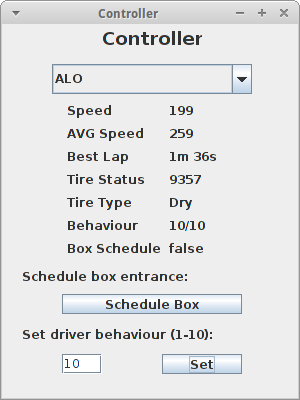
\includegraphics[keepaspectratio = true, width = 200px] {Pictures/controller}
		\rule{35em}{0.5pt}
	\caption[Controller]{Controller: Dati aggiuntivi e strumenti per modificare alcuni parametri.}
	\label{fig:Controller}
\end{figure}

Il controller è l’elemento che permette all’utente di interagire con l’andamento della gara. L’idea di base è quella di fornire un controllo simile a quello che possono avere i box, e quindi restare su un livello prettamente strategico.
Siccome è impensabile far fare scelte che richiedano tempi di risposta troppo veloci ad un giocatore inesperto, abbiamo deciso di fornire all’utente solamente la possibilità di manipolare decisioni che abbiano valenza anche se vengono prese in considerazione dopo un breve tempo di attesa.
L’idea alla base dell’implementazione del controller è abbastanza simile a quella del monitor, anche se è semplificata dal fatto di non avere i vincoli di refresh necessari alla rappresentazione.
Come prima cosa, viene richiesto il setup al broker, passo necessario per ottenere le informazioni sul numero di veicoli partecipanti. Come per il monitor, i veicoli vengono identificati nei messaggi solo da un numero, e la loro traduzione con il nome del pilota viene effettuata tramite lo stesso file utilizzato dal monitor per la classifica.
Dato il diverso tipo di comunicazione è stata implementata una nuova classe per la sua gestione, chiamata ControllerCommunicator.java. Questa classe è profondamente diversa da quella vista precedentemente nel monitor, infatti i dati non vengono più ricevuti in subscribe dal broker, ma devono essere richiesti (pull); questo implica che non è più una entità attiva che raccoglie i dati, ma diventa un’entità passiva che invia richieste solo quando necessario.
Il suo compito non si limita a fare richieste in pull tramite il metodo “getDetail”, ma comprende anche l’invio dei messaggi di override al core, tramite i metodi “overrideBehaviour” e “overrideBoxEntrance”.
Successivamente viene inizializzato un oggetto della classe ControllerWindow.java, che contiene il pannello della finestra, su cui vengono mostrate le varie informazioni.
Nella finestra è possibile scegliere un veicolo dalla lista, e da quel momento verranno visualizzati i dettagli relativi alla macchina, e ogni istruzione inviata si riferirà a quella specifica vettura.
Al termine della gara la finestrà non si chiude, ma avvisa l’utente che la connessione è stata interrotta; solo alla chiusura della finestra viene chiuso definitivamente il controller.
Come per il monitor, l’avvio e la relativa connessione possono essere effettuati in qualsiasi momento, non necessariamente all’avvio della gara.

\subsection{Eventi}

Come già accennato precedentemente, la simulazione nel core generea un flusso continuo di eventi che vengono poi inviati all’intermediario. Gli eventi sono composti da un numero variabile di coppie chiave-valore, diverse per ogni tipo. Vediamo ora in dettaglio la loro composizione:

Fine Segmento: \\
   type = ES $|$ car = (Pos)ID $|$ seg = (Pos)Seg\textunderscore ID $|$ vel = (Int)speed $|$ beh = (Pos)behaviour $|$
   tire\textunderscore s = (Int) tire\textunderscore status $|$ tire\textunderscore t = (bool)rain\textunderscore tire $|$ time = (time\textunderscore span) $|$ r\textunderscore box =(bool)request\textunderscore box

Rientro ai box: \\
   type = EB $|$ car = (Pos)ID $|$ time = (time\textunderscore span)

Uscita dai box: \\
  type = LB $|$ car = (Pos)ID $|$ tire\textunderscore t = (bool)rain\textunderscore tire $|$ lap = (Pos)giro terminato $|$ time = (time\textunderscore span)

Fine Giro: \\
  type = EL $|$ car = (Pos)ID $|$ lap = (Pos)giro terminato $|$ time = (time\textunderscore span)

Una macchina conclude la gara: \\
  type = CE $|$ car = (Pos)ID $|$ time = (time\textunderscore span)

La gara è finita: \\
  type = ER

Una macchina fa un incidente: \\
  type = CA $|$ car = (Pos)ID $|$ damage = (bool) $|$ retired = (bool) $|$ seg = (Pos)segmento $|$
  time = (time\textunderscore span)

Cambio meteo: \\
   type = WC $|$ rain = (bool)

Setup: \\
  type = SE $|$ ncar = (Int)real\textunderscore car\textunderscore number $|$ nlap = (int)real\textunderscore laps\textunderscore number
  
\subsection{Snapshot}

Gli eventi sopracitati, vengono tradotti dall’intermediario in uno snapshot, ovvero una fotografia dello stato della gara in un dato istante. Come già detto, ce ne sono di due tipi: lo snapshot generalista e quello dettagliato.
Lo snapshot generalista contiene una riga per ogni macchina, ed è composta da:

\begin{itemize}
 \item lap(Integer) = numero di giro di pista corrente
 \item segment(Integer) = identificativo del segmeno in cui è correntemente (-1 per il box)
 \item progress(Float) = percentuale di completamento del segmento corrente
 \item incident(Boolean) = indica che sta facendo un incidente, è fuori pista
 \item damaged(Boolean) = indica se è danneggiata
 \item retired(Boolean) = indica se si è ritirata
 \item over(Boolean) = indica se ha finito la corsa
 \item ranking(Integer) = indica la sua posizione in classifica
\end{itemize}

Nello snapshot dettagliato troviamo invece, per ogni macchina:

\begin{itemize}
 \item tire\textunderscore status(Integer) = livello degli pneumatici
 \item rain\textunderscore tires(Boolean) = indica se monta gomme da pioggia
 \item average\textunderscore speed(Float) = la media di velocità tenuta da inizio corsa
 \item behaviour(Integer) = il comportamento che tiene il pilota, da 1 a 10
 \item current\textunderscore speed(Integer) = la velocità attuale
 \item require\textunderscore box(Boolean) = indica se ha richiesto una sosta ai box
\end{itemize}